\section{McCulloch-Pitts-Neuron} \label{sc:mpn}

\subsection{Funktionsweise}

Im Jahr 1943 entwickelten Warren McCulloch und Walter Pitts ein Modell das die Funktionalität eines biologischen Neurons imitieren sollte. In der folgenden Abbildung \ref{fig:bioNeuron} ist der grobe Aufbau eines biologischen Neurons zu sehen. 

\begin{figure}[!htb]
	\centering
	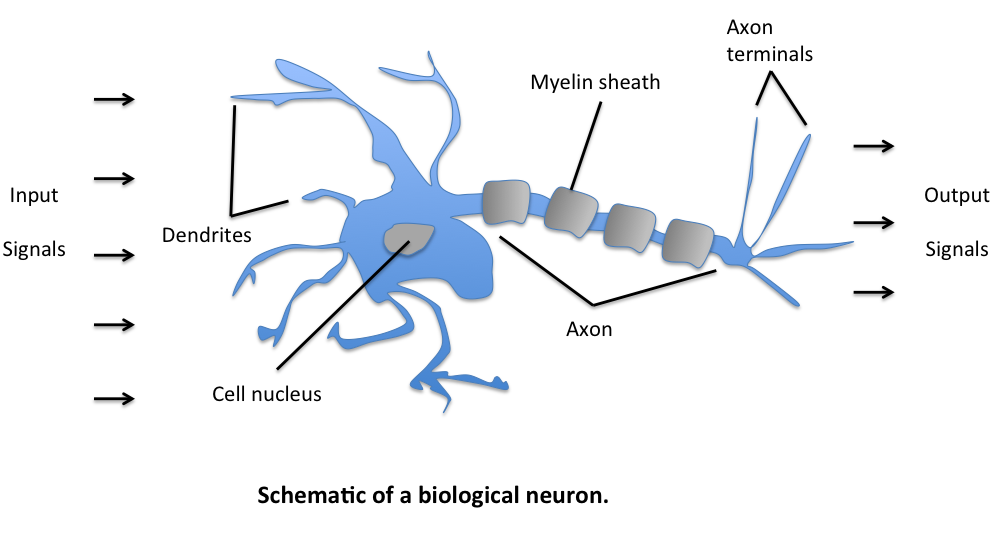
\includegraphics[width=\linewidth]{img/bioNeuron}
	\mycaption{McCulloch-Pitts-Zellne - Genereller Aufbau}{mpNeuron}
	\label{fig:bioNeuron}
\end{figure}

Die sogenannten \emph{Dendriten} (englisch \emph{dendrites}) nehmen Informationen auf. Sie besitzen Rezeptoren welche in der Lage sind Signale anderer Neuronen aufzunehmen. Diese Signale bewirken elektrische Veränderungen in dem Neuron welche vom Zellkörper (\emph{Soma}) interpretiert / verarbeitet werden. Dieser Zellkörper sammelt alle Informationen und speichert diese im sogenannten \emph{Axonhügel} (engl. Axonhillock) welcher die Ursprungsstelle des \emph{Axons} beziehungsweise der \emph{Neuriten} beschreibt. Wenn das gebündelte Signal stark genug sein sollte, wird es an den nächsten Teil des Neurons (dem \emph{Axon}) weitergeleitet. Ab diesem Zeitpunkt wird das Signal als \emph{Aktionspotential} bezeichnet und wird über die \emph{Axon} übertragen. Am Ende wird das Signal an diverse \emph{Axonterminale} weitergeleitet welche per Neurotransmitter mit den jeweils nächsten Dendriten verbunden sind. 

Dieser biologische Aufbau dient als Grundlage für die Entwicklung des Modells von McCulloch und Pitts. Das Augenmerk ihres Modells liegt in erster Linie darauf Klassifizierungsprobleme zu lösen. Bei einem Klassifizierungsproblem wird \emph{das zu klassifizierende Objekt X ist dabei durch einen Merkmalvektor $\vec{x}$ aus dem betrachteten Merkmalraum M mit der Dimension n charakterisiert. Das Problem besteht nun darin zu entscheiden, ob das Objekt X in der betrachteten Klasse K liegt.} \cite{klproblem}. Der grobe Aufbau einer sogenannten \emph{McCulloch-Pitts-Zelle} ist in Abbildung \ref{fig:mpn_aufbau} zu sehen. Erwähnt sei ebenfalls, dass man mit diesem Modell lediglich binäre Klassifizierungen mittels einer linearen Entscheidungsfunktion / Aktivierungsfunktion durchführen kann (siehe \ref{fig:aufbau})


\begin{figure}%
  \centering
  \subfloat[][]{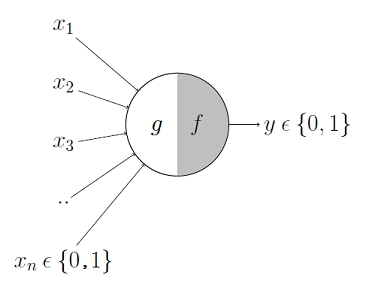
\includegraphics[width=.4\linewidth]{img/aufbau}}
  \qquad
  \subfloat[][]{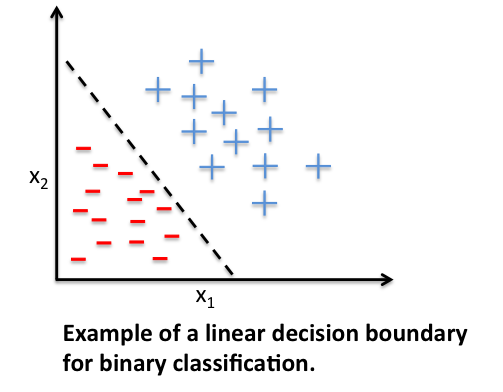
\includegraphics[width=0.4\linewidth]{img/bnKlassifizierung}}%
  % todo zweite Quelle mit in Macro einbinden
  \mycaption{McCulloch-Pitts-Zelle: Aufbau und Klassifizierung}{mpNeuron}
  \label{fig:aufbau}
\end{figure}

Das Modell kann beliebig viele Eingabe-Werte aufweisen. Wichtig hierbei: Sie dürfen nur boolescher Natur sein (nur falsch oder wahr). Bei gegebenen Werten führt das Neuron selbst zwei Arbeitsschritte durch: 
\begin{enumerate}

\item Erst werden alle Werte aufaddiert (in der Abbildung dargestellt durch die Funktion \emph{g}). Dies imitiert das Verhalten der \emph{Dendriten} in einem biologischen Neuron. 

\item Anschließend überprüft die Funktion \emph{f} ob ein gegebener Schwellwert überschritten wurde oder nicht (gibt dies entsprechend in Form einer booleschen Ausgabe weiter). Das biologische Neuron tut dies mittels des \emph{Axonhügels}. 

\end{enumerate}

Die übliche Notation dieses Modells gibt vor, dass der jeweilige Schwellwert jeweils in die linke Seite des Kreises geschrieben, während die rechte Seite ausgegraut wird. Im folgenden seien einmal beispielhaft das \emph{AND} und das \emph{OR} Gatter dargestellt. (Für weitere Beispiele siehe \autoref{ap:sc:mpz})

\begin{figure}[!htb]
	\centering
	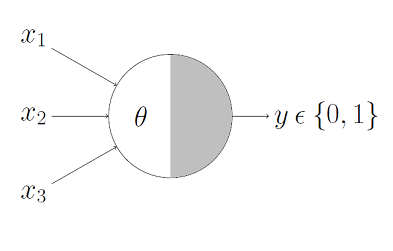
\includegraphics[width=.4\linewidth]{img/aufbau2}
	\mycaption{MPZ - Notation}{mpNeuron}
	\label{fig:mpn_aufbau}
\end{figure}

\begin{figure}[!htb]
	\centering
	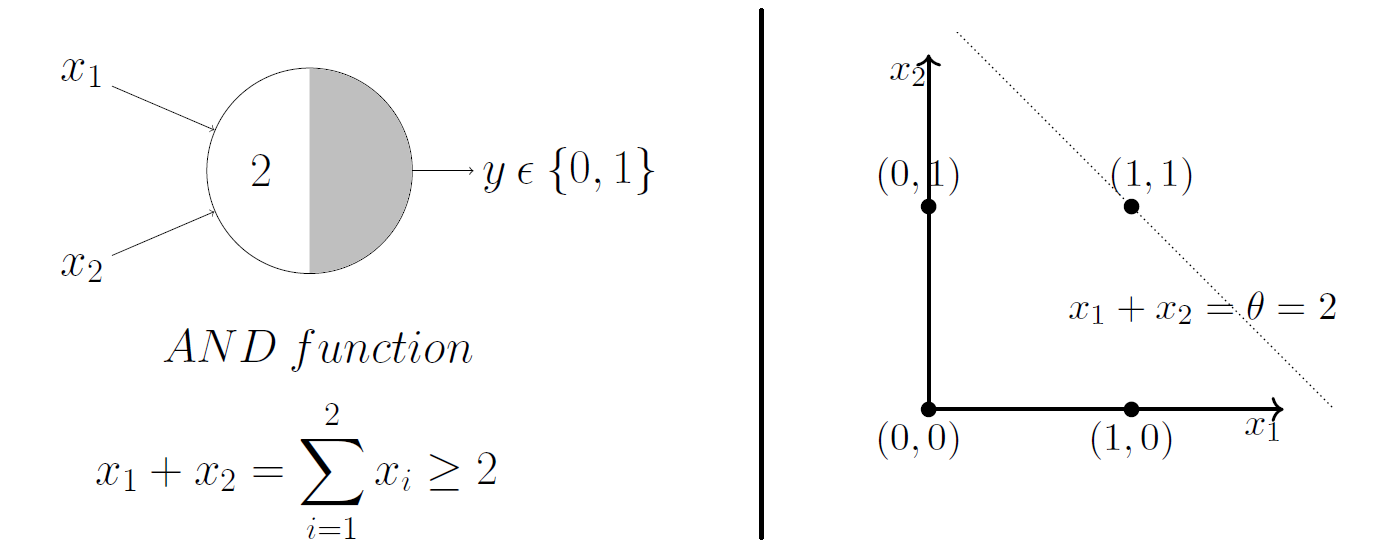
\includegraphics[width=.8\linewidth]{img/mpn_and}
	\mycaption{McCulloch-Pitts-Zelle - AND Gatter}{mpNeuron}
	\label{fig:mpn_and}
\end{figure}

\begin{figure}[!htb]
	\centering
	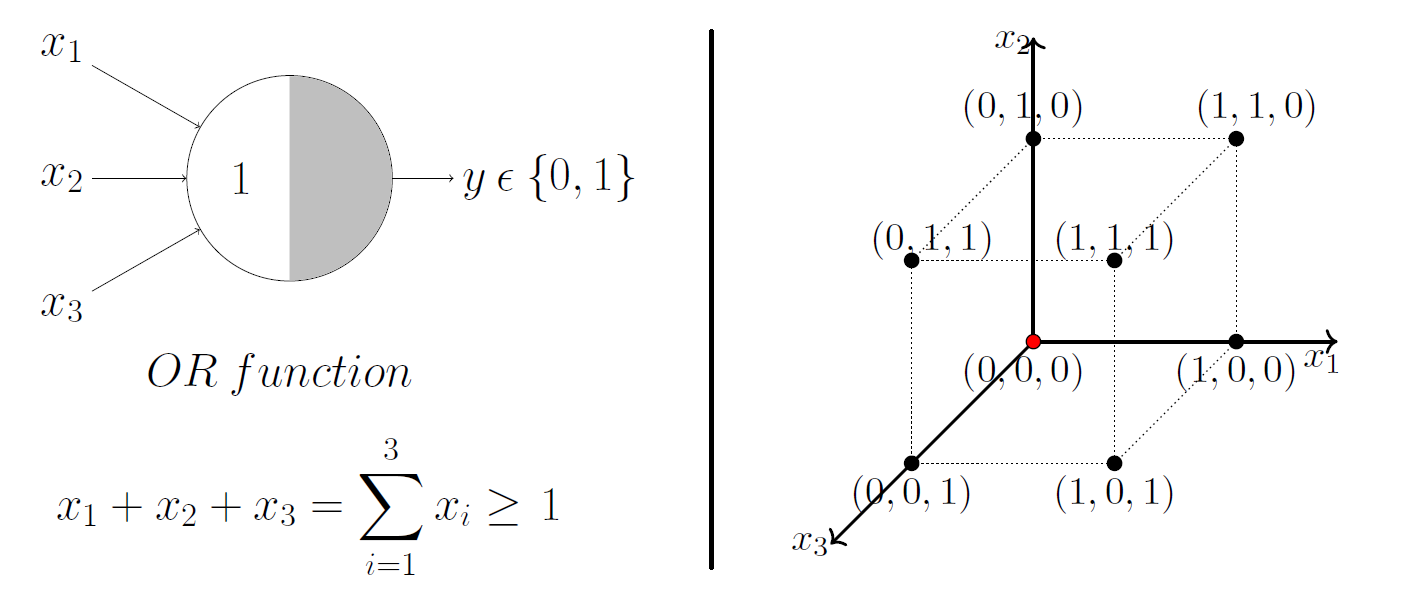
\includegraphics[width=.9\linewidth]{img/mpn_or}
	\mycaption{McCulloch-Pitts-Zelle - OR Gatter}{mpNeuron}
	\label{fig:mpn_or}
\end{figure}


\subsection{Nachteile bzw. Verbesserungspotenzial}

\begin{minipage}{\textwidth}
\begin{itemize}

\item Dieses Modell  nur boolesche Eingabewerte, viele Modelle erfordern allerdings kontinuierliche Werte. Mit diesen wäre es zum Beispiel deutlich einfach ein Bild oder Ähnliches zu analysieren.

\item Die Schwelle (Theta) muss stets manuell bestimmt werden. Einen Trainingsalgorithmus wie man ihn von heutigen Ansätzen her kennt gibt es in diesem Modell nicht. 

\item Es gibt keinerlei Priorisierungsmöglichkeit zwischen den einzelnen Eingabewerten. Jeder hat einen gleichgroßen Einfluss auf das Ergebnis, so etwas wie ein Auschlußkriterium gibt es hierbei also nicht. 

\item Es ist nicht möglich \emph{gedeckelt} Gatter wie zum Beispiel ein \emph{XOR} abzubilden. Bei einem Neuron mit zwei Eingabe-Werten müsste zum Beispiel ein Schwellwert von 1 \underline{genau} getroffen werden. Dieses Modell ist allerdings nur in der Lage zu entscheiden ob ein Schwellwert \emph{überschritten} wurde oder nicht. 

\end{itemize}
\end{minipage}

